\subsection{Parameter Tuning}

To test the performance of the decision tree the raw data set of person G3M2 was used.
A 90/10\% split was performed on the data.
In the following sections a series of tests are made to find the optimal of all prepossessing methods.

% - what are decision trees
% - limiting pruning (confidence factor) control=C5.0Control(CF= seq(0,1,0.1))
% - Must have at least minimum number of cases to use as decision split. C5.0Control(minCases=2:10)
% - winnow algo \(\sum_{i=1}^{n} w_i x_i > \Theta\), C5.0Control(winnow = TRUE)
% 
% The idea of a decision tree is to split the classifications into a set of decisions.
% The first 50 PCA values are used and by looking at the deviance for each split a tree can be created.
% 
% winnow = good,
% minimum cases = use as example
% 
% 
% 
% 
% using datasets: all mixed 5 + 5

\subsubsection{Raw Performance}

To find a baseline of the prepossessing impact, a test on the raw data was performed.
The minimum number of cases was increased to see its effect on the performance on the tree.
The results of this test can be seen in figure \ref{fig:tree_raw}. 
The optimal minimum number of cases were found to be 7 and thus used in the following tests.

\begin{figure}[H]
\centering
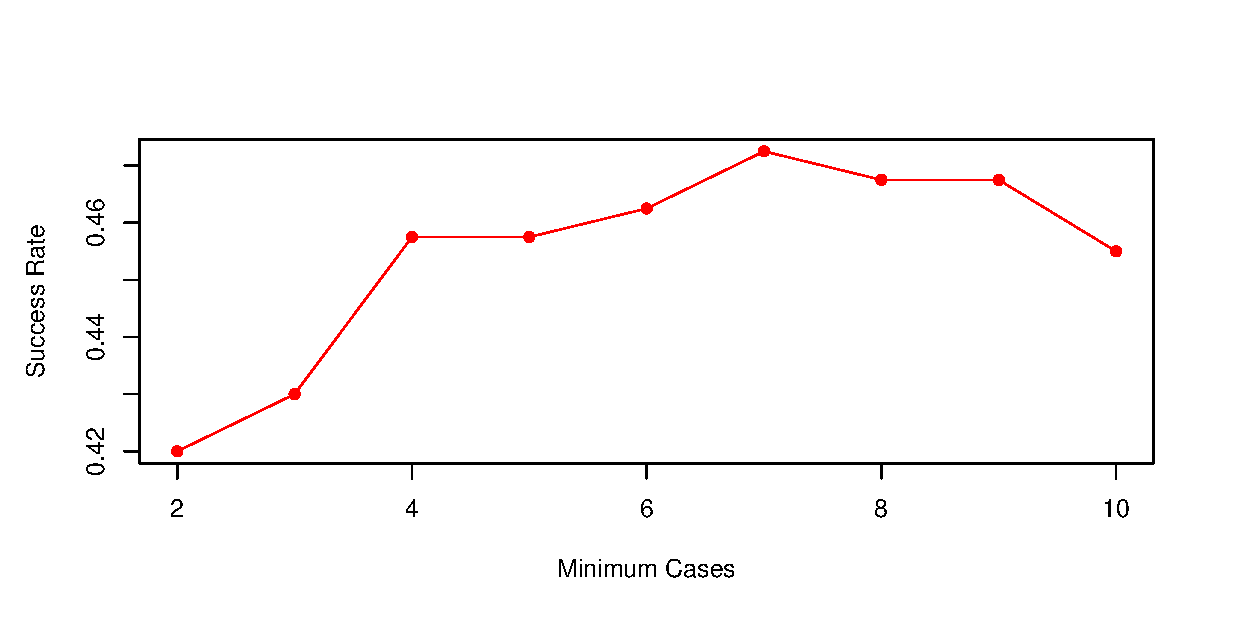
\includegraphics[width=0.7\textwidth]{graphics/tree_raw}
\caption{Raw performance of decision tree. Minimum number of cases used to make a decision. }%Tested with person 3.2 using a 90/10 split}
\label{fig:tree_raw}
\end{figure}


\subsubsection{Smoothing}

Smoothing of the image was done with the Gaussian smoothing filter as discussed in section \ref{sec:smoothing}.
The tree was built with the minimum number of 7 cases.
The success rate of the decision tree with the filter is shown in figure \ref{fig:tree_smooth}.
To find the optimal kernel size and variance, the effects on both were plotted.
A large kernel size does not impact the low variance. The optimal kernel size were found at    7
% while the optimal variance was found at                                                        0.9.

\begin{figure}[H]
\centering
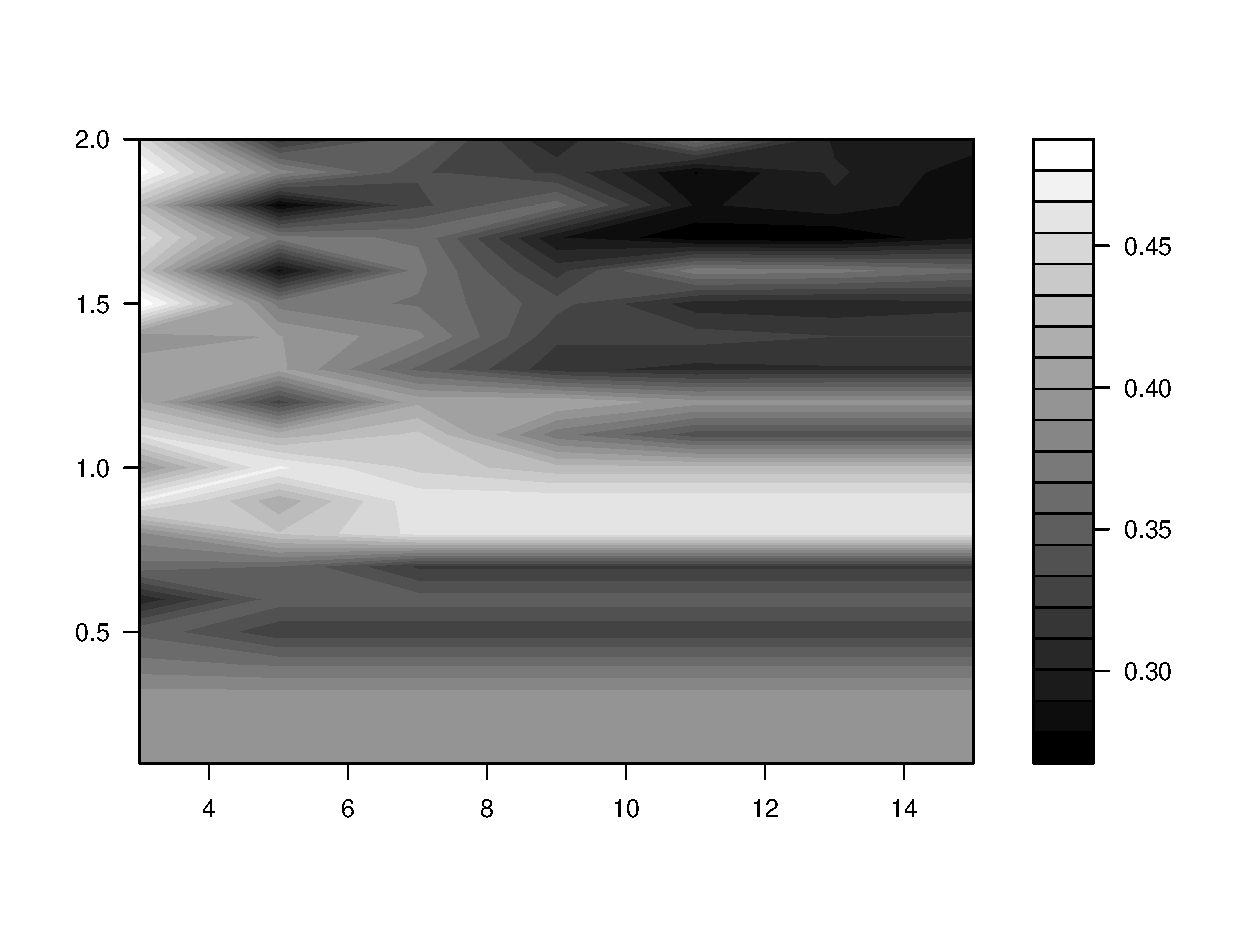
\includegraphics[width=0.7\textwidth]{graphics/tree_smooth}
\caption{Gaussian smoothing on image as pre-processing. Kernel size vs $\sigma$. }%Tested with person 3.2 using a 90/10 split}
\label{fig:tree_smooth}
\end{figure}

\subsubsection{Principle Component Analysis}

To find the optimal number of principle components to use in a decision tree 
% both 
the smoothed data 
% and raw data 
was tested.
The optimal number of principle components was chosen as 130.

\begin{figure}[H]
\centering
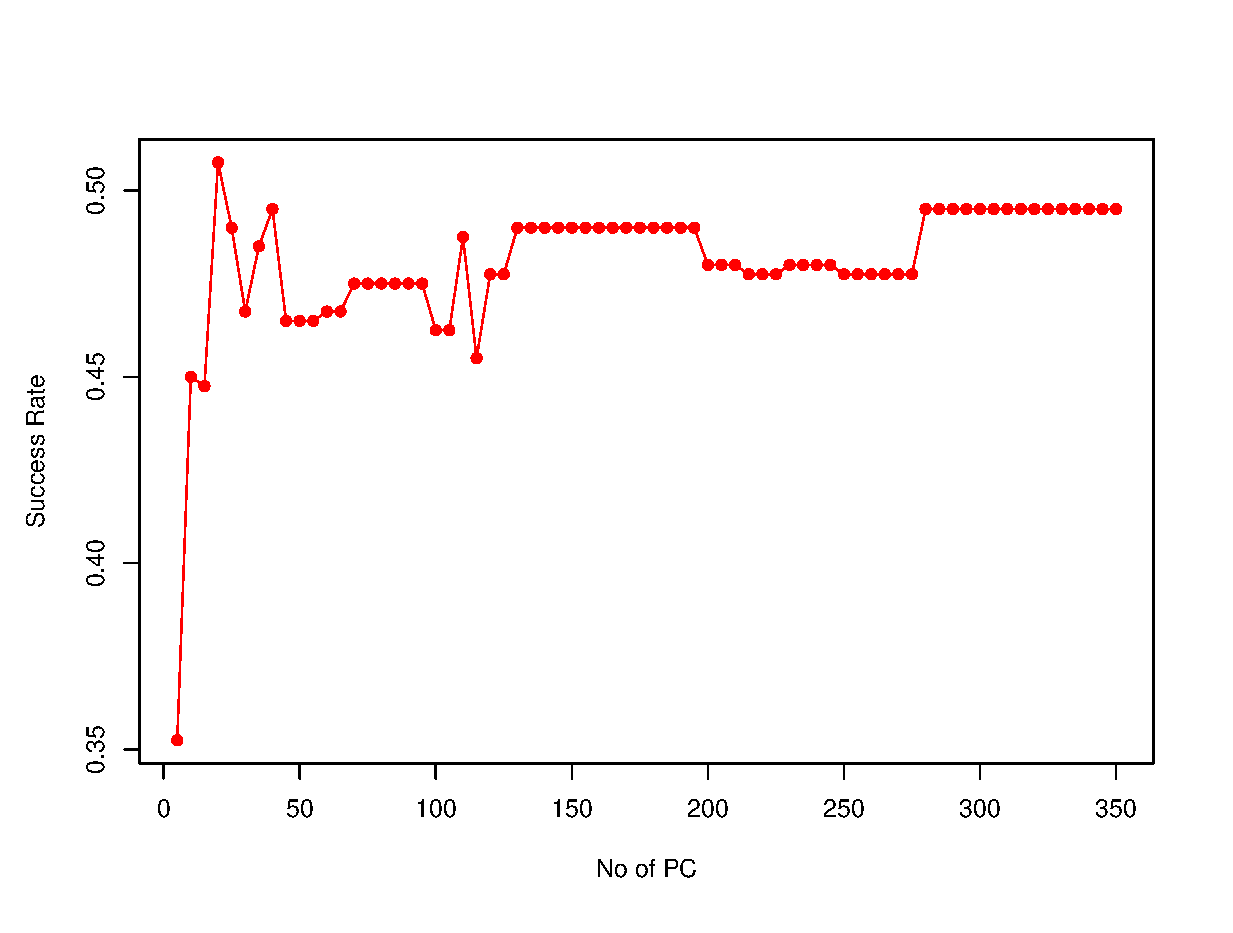
\includegraphics[width=0.7\textwidth]{graphics/tree_pca}
\caption{Sigma/size vs PC or success vs PC if best smoothing distinct.}
\end{figure}


\subsubsection{Combinations}

To test the combinations of the methods all were plotted using the found optimal settings.
Smoothing (S), Z-Score (ZS), and PCA was applied on the data.
The first result is the raw data.
In figure \ref{fig:tree_total} the success rate with the different methods is applied.

\begin{figure}[H]
\centering
% \missingfigure{qwe}
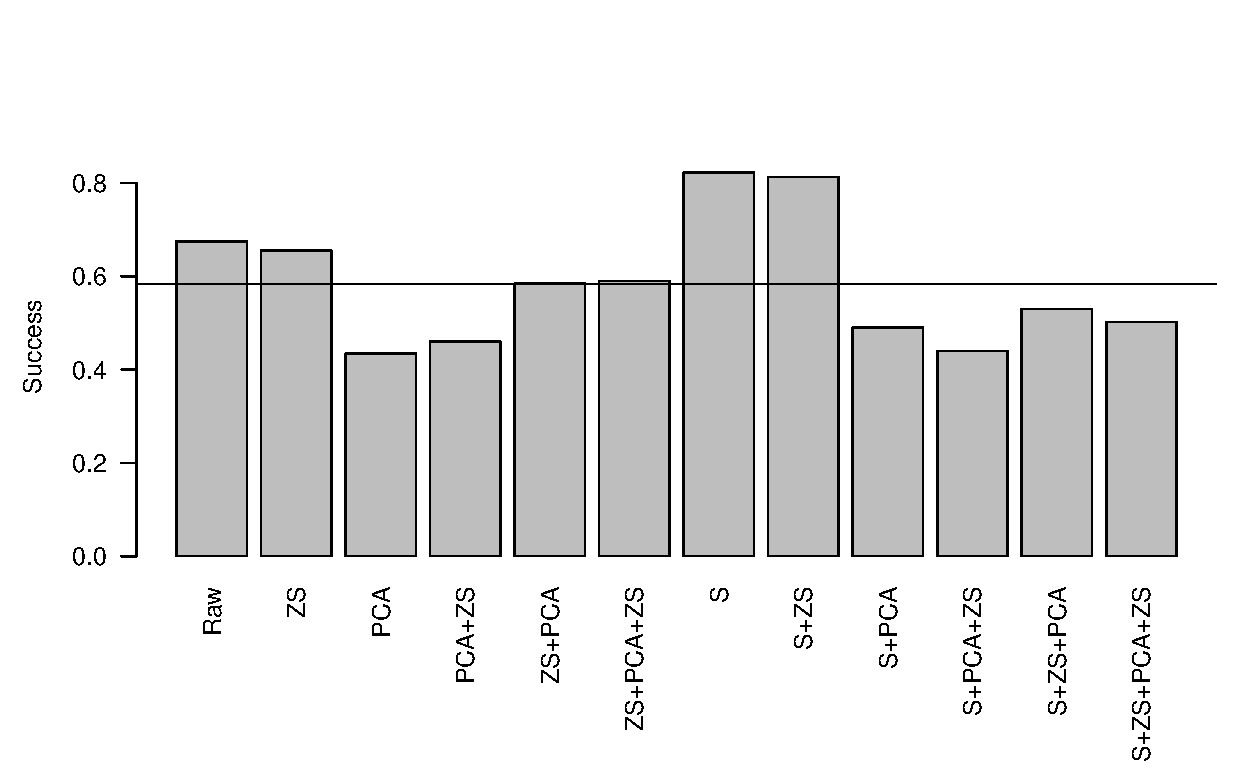
\includegraphics[width=0.7\textwidth]{graphics/tree_total}
\caption{Success for raw, pre zs, post zs and both.}
\label{fig:tree_total}
\end{figure}

To test on a larger data set the same tests were performed on a mix of 20 peoples data where 100 digits of each class were used as training and 50 digits of each class was used for testing.
In figure \ref{fig:tree_total_mixed} is the results shown.
While the overall performance has gone down the impact of each method is similar.

\begin{figure}[H]
\centering
% \missingfigure{qwe}
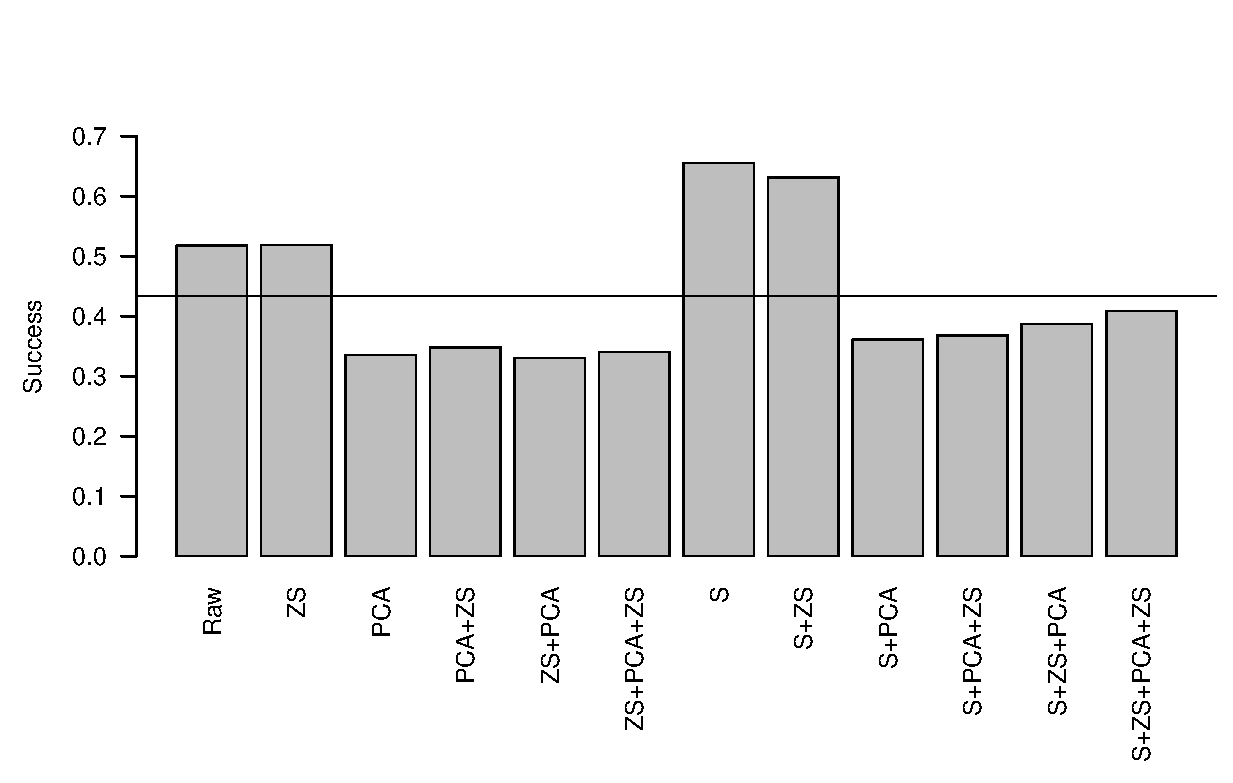
\includegraphics[width=0.7\textwidth]{graphics/tree_total_mixed}
\caption{Success for raw, pre zs, post zs and both.}
\label{fig:tree_total_mixed}
\end{figure}

In figure \ref{fig:tree_total_all} is the tree trained with 19 people's data. 
Of each member was 50 digits chosen.
G3M2 was taken out of the training data and used to test the methods.
From these tests it can be concluded that simply smoothing the data gives the best result.
Applying PCA will decrease the performance although applying Z-Score on the data before improves the PCA.
Therefore the optimal prepossessing must be smoothing the data, normalizing with Z-Score and reduce the data set with PCA.
Normalizing the data after the PCA gave a better performance on the test with the mixed data but the two other tests showed the opposite.

\begin{figure}[H]
\centering
% \missingfigure{qwe}
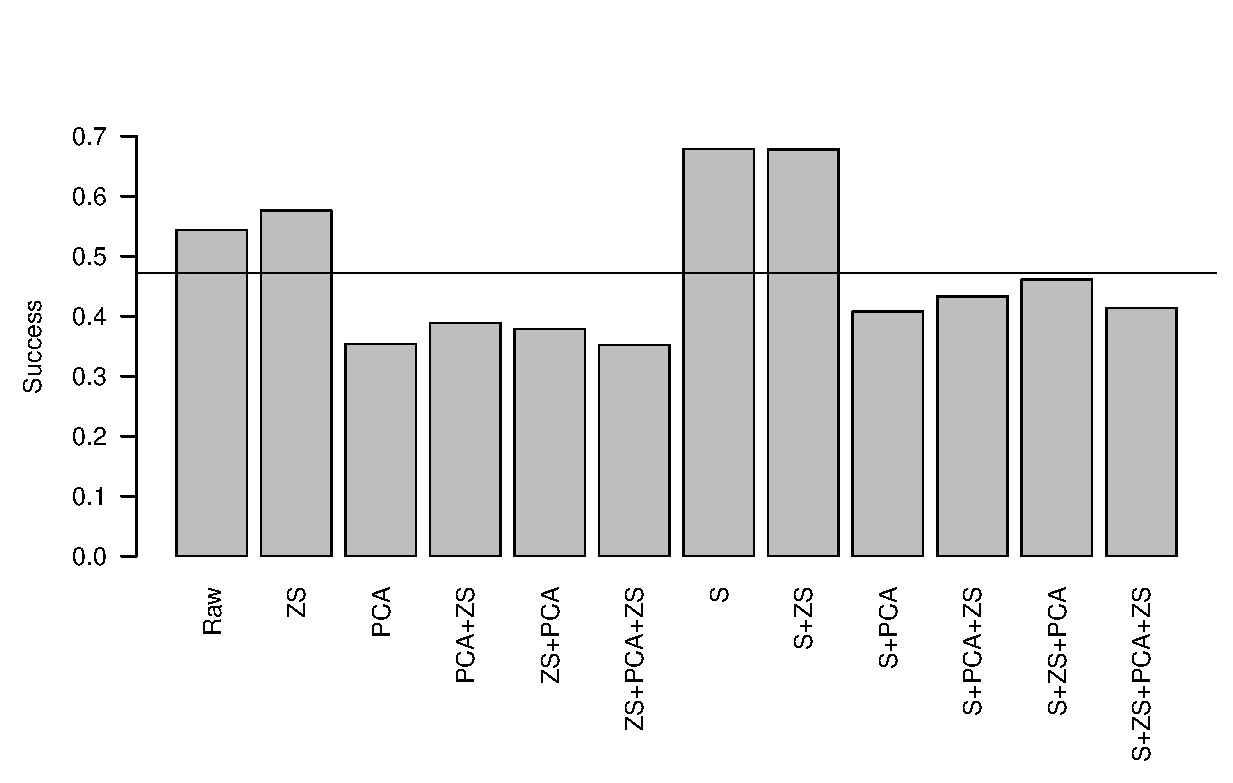
\includegraphics[width=0.7\textwidth]{graphics/tree_total_all}
\caption{success for raw, pre zs, post zs and both}
\label{fig:tree_total_all}
\end{figure}

\subsubsection{Boosting}
Boosting is a process in which the algorithm is training with the train data with multiple trials to increase performance.
Boosting works by comparing the information gain of each subtree and use the best method for the final tree.
Because the optimal decision path is unknown until every decision split is made, boosting makes multiple trees and compares the performance.
While the performance can only be measured on the data available (the training data) the model can be fitted to perform well on the errors in the training data and thus potentially decrease the performance on the test data.
This is called overfitting. 
In figure \ref{fig:tree_overfitting} the boosting of the training set and the test set can be seen.
It can be seen that after a few boosts the model gains a 100\% success rate on the training data.
Therefore it cannot know what to improve upon and the performance cannot be better on the test data.

\begin{figure}[H]
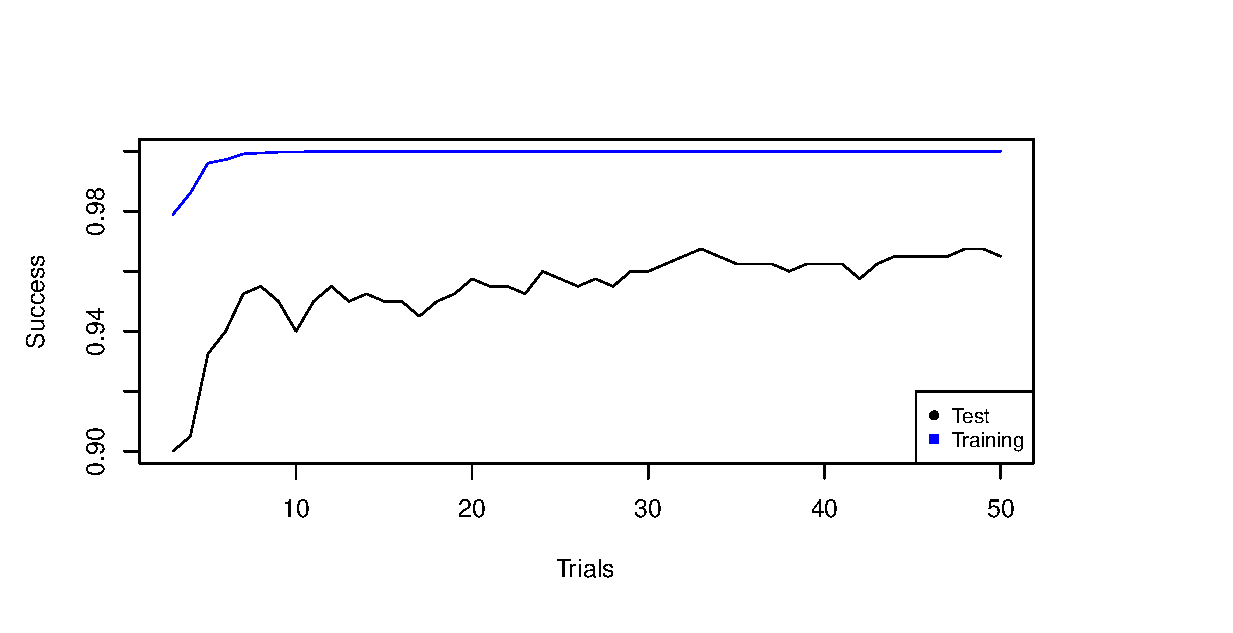
\includegraphics[width = \textwidth]{graphics/tree_boost_overfitting}
\caption[Boosting decision tree]{Performance of boosting the C50 algorithm. 
The tree is trained on the data from person G3M2. 
When the performance on the train data hits 100\% the performance on the test data fluctuates. }
\label{fig:tree_overfitting}
\end{figure}

The ``C50'' function provides a boosting function.
In figure \ref{fig:tree_timing} can the success be seen of multiple trials.
Since the algorithm trains towards a good performance on the train data it can not improve beyond a certain point.
The ideal number of boosting trails is set to 7.
The timing is as expected linear dependent on the number of trials.

\begin{figure}[H]
% 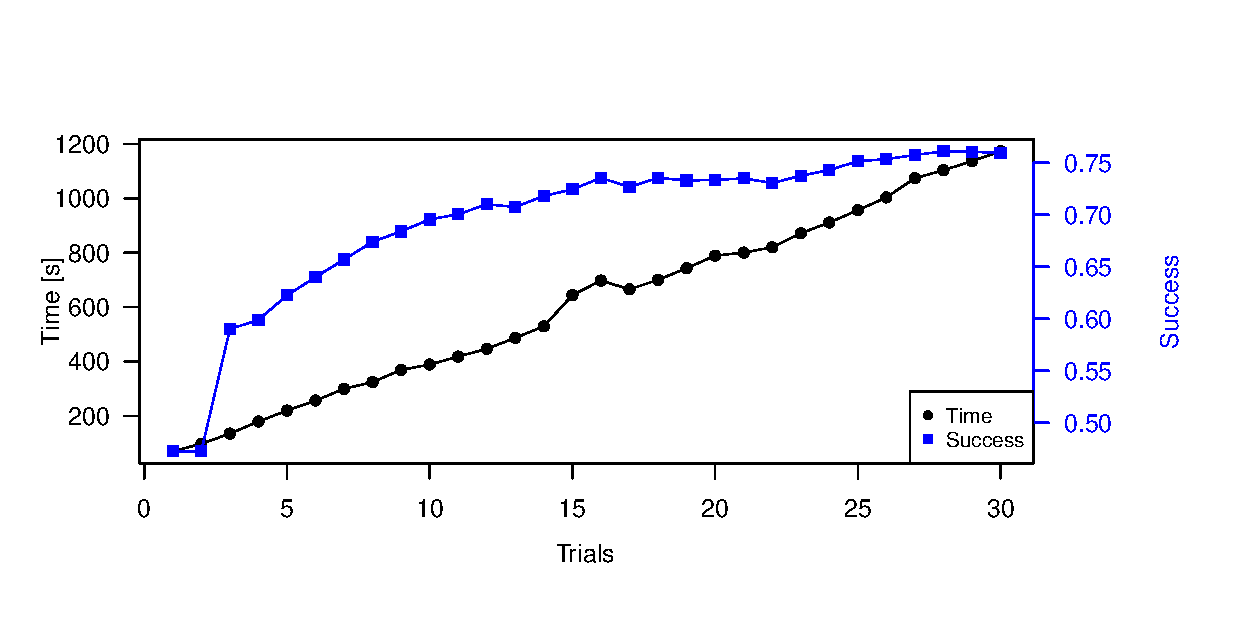
\includegraphics[width = \textwidth]{graphics/tree_timing}
% 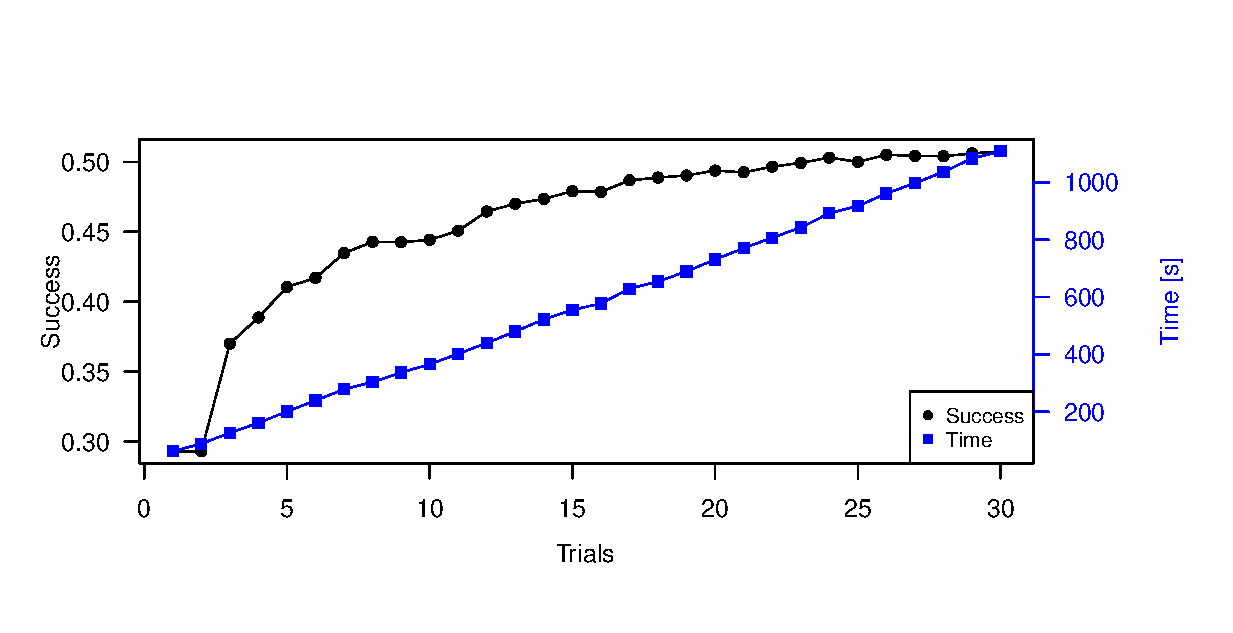
\includegraphics[width = \textwidth]{graphics/tree_timing_entropy}
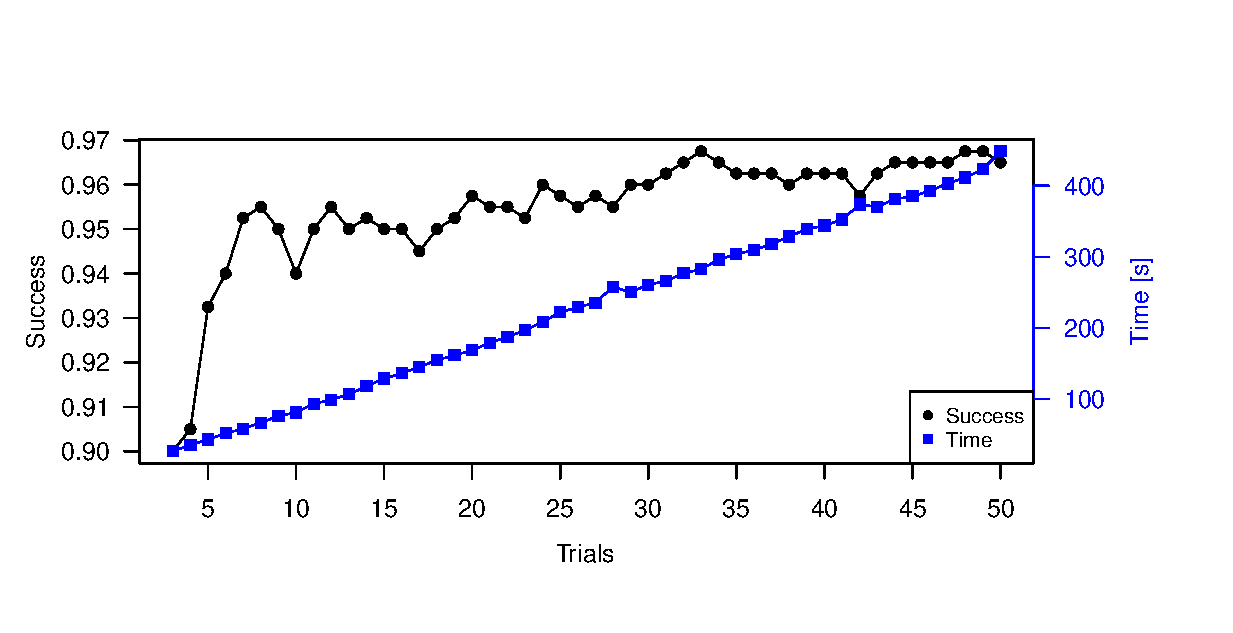
\includegraphics[width = \textwidth]{graphics/tree_timing_one}
\caption[Timing of the boosting function.]{Timing of the boosting function.}
\label{fig:tree_timing}
\end{figure}

Since the performance increases with the timing it could be expected to improve the performance of a reduced data set.
In figure \ref{fig:tree_pca_boost} is the performance shown with an increasing number of trials and an increasing number of PC.

It can be seen that a combination of 75 PC and 24 trials gives the best result.

\begin{figure}[H]
\centering
    \begin{subfigure}[t]{0.49\textwidth}
        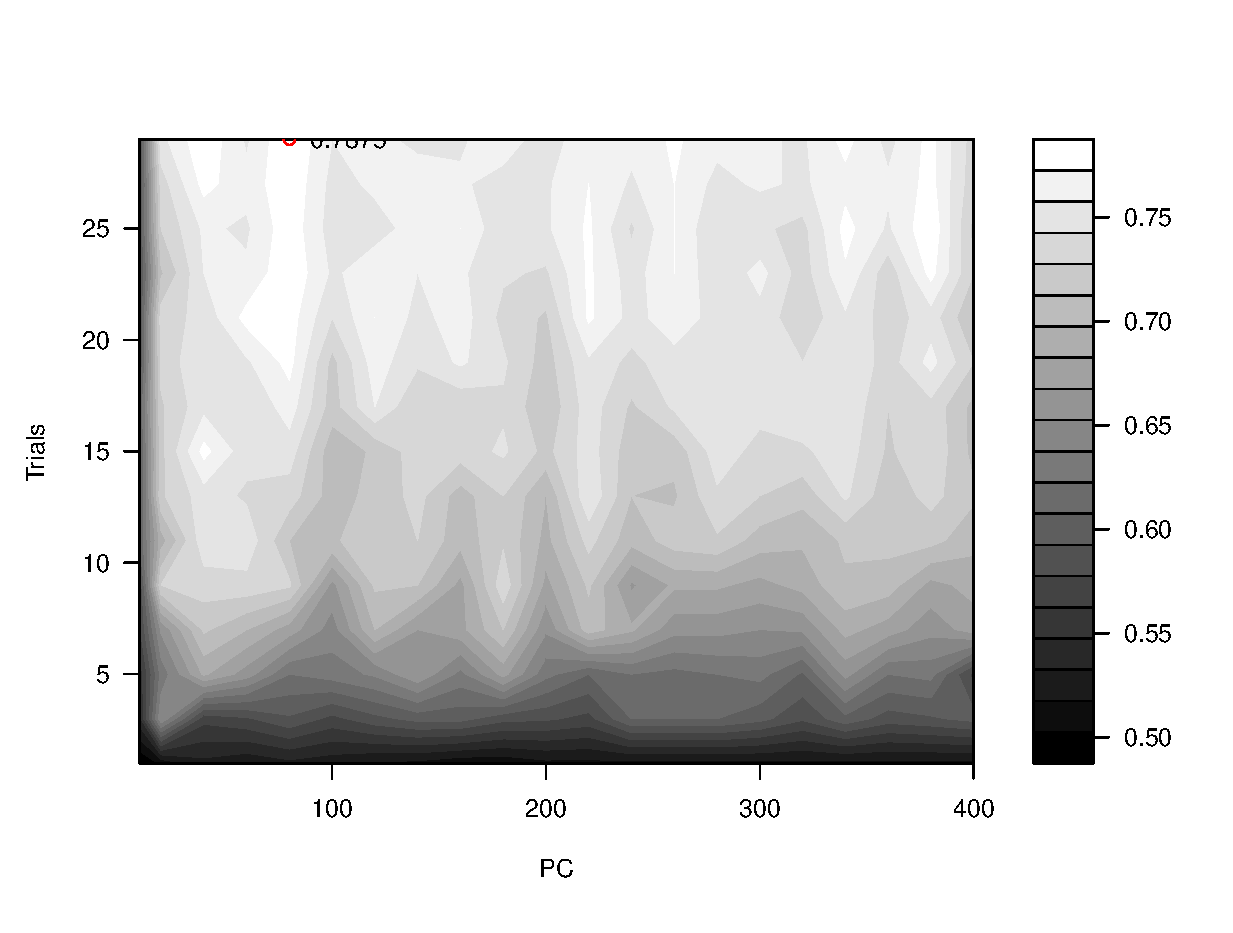
\includegraphics[width=\textwidth]{graphics/tree_pca_vs_boost_success}
        \caption{Success of boosting the tree.}
        \label{fig:tree_pca_boost}
    \end{subfigure}
    \begin{subfigure}[t]{0.49\textwidth}
        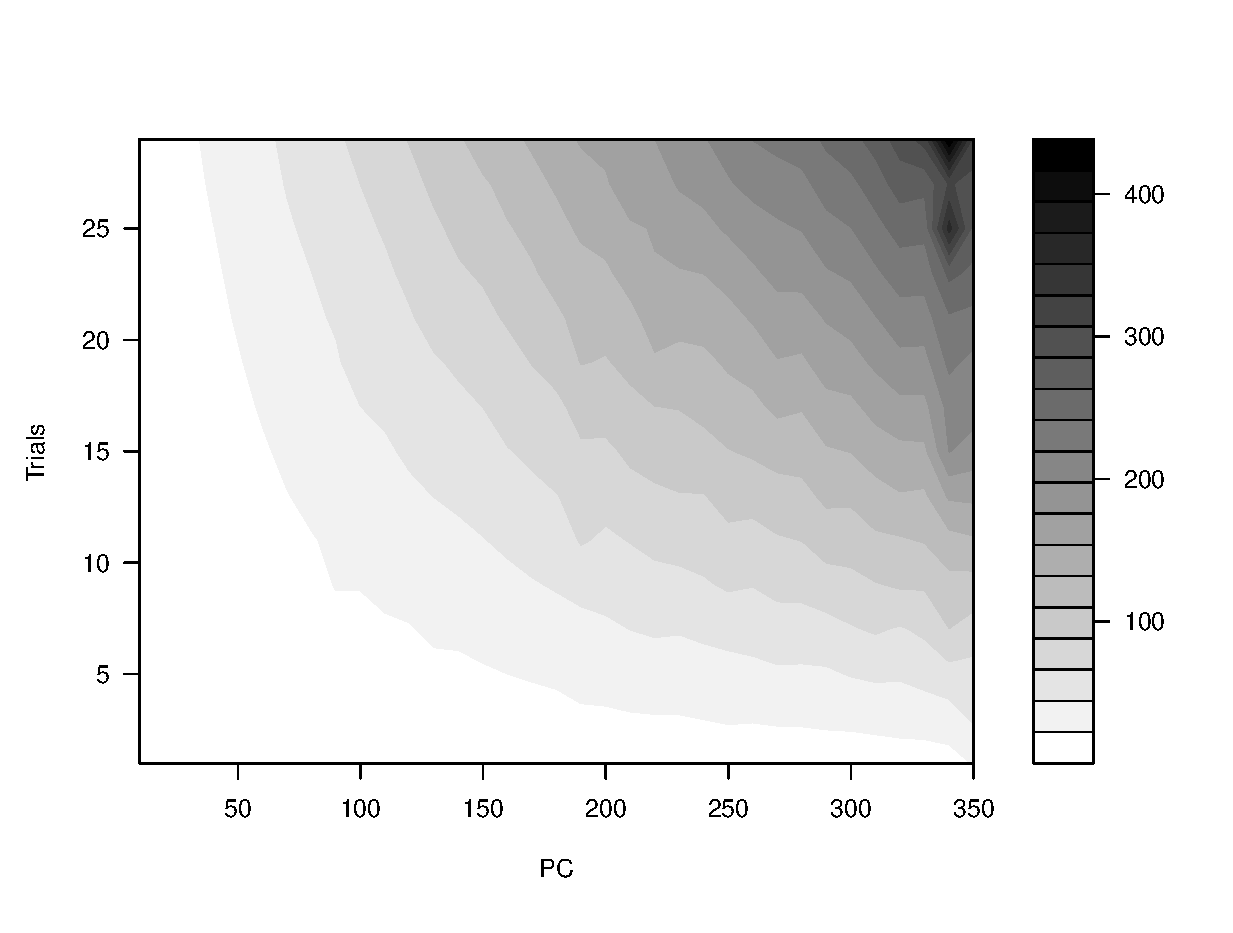
\includegraphics[width=\textwidth]{graphics/tree_pca_vs_boost_time}
        \caption{Time of boosting the tree.}
        \label{fig:tree_pca_boost_timing}
    \end{subfigure}
\caption{Number of PC used vs boosting trials on decision tree.}
\label{fig:tree_pca_boost}
\end{figure}

To find the optimal balance between reducing the dataset with PCA and optimizing the performance with boosting the timing of the functions were measured.
In figure \ref{fig:tree_pca_boost_timing} is the time it took to build the tree shown.

\subsubsection{Performance}

\begin{table}[h]
\centering
\begin{tabular}{lr}
min. nodes  & 7      \\
z-score     & before \\
PC          & 75     \\
Trials      & 24     \\
sigma       & 0.9    \\
kernel size & 7      \\
\end{tabular}
\caption{Optimal Parameters for decision tree.}
\label{tb:tree_simply_the_best_parameters}
\end{table}


In table \ref{tb:tree_simply_the_best_parameters} is the optimal parameters shown.
These parameters are applied to the prepossessing and tree function. 
This data set is referred to as the prepared data set.
To test these against the data 20 peoples data have been mixed.
90\% of the data was used to train the tree and 10\% were used to test the performance.
This was done running 10 cross-referencing tests. 
To compare the results with the smoothed data and no prepossessing the same training set was used.
Here the number of boosting trials was set at 7. 
This data set is referred to as the smoothed data set.
The results can be seen in figure \ref{fig:tree_performance_mixed}.
To see how each digit was detected a confusion table is shown in figure \ref{fig:tree_confus_mixed}. 
Here it is seen that while 8 has a high correct detection rate, outliers of other numbers is more likely to be classified as an 8.

\begin{figure}[H]
\centering
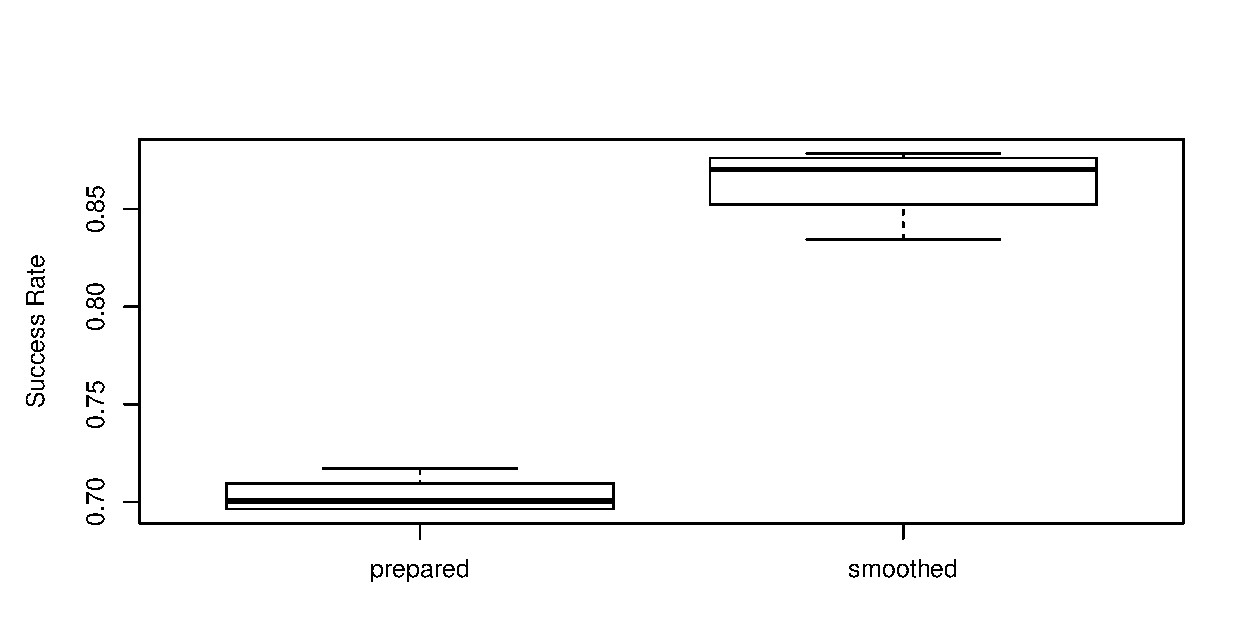
\includegraphics[width=\textwidth]{graphics/tree_performance_mix_combined}
% 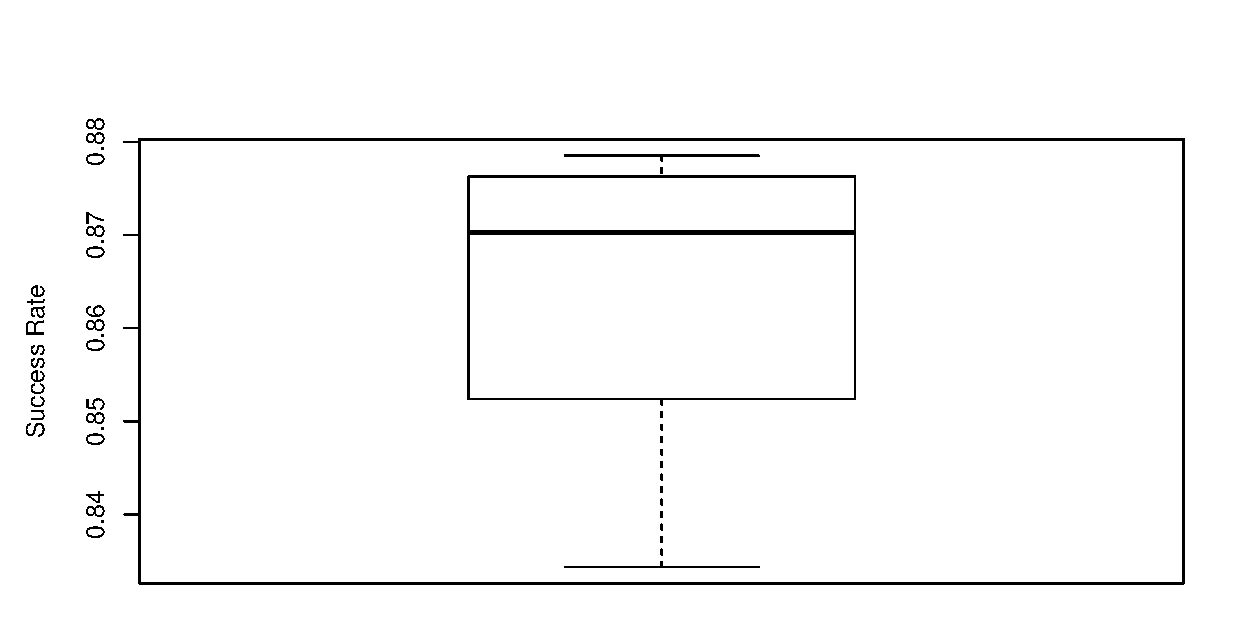
\includegraphics[width=0.49\textwidth]{graphics/tree_performance_mix2}
\caption{Success rate with all the best parameters for the full dataset easy problem.}
\label{fig:tree_performance_mixed}
\end{figure}

\begin{figure}[H]
\centering
\begin{subfigure}{0.49\textwidth}
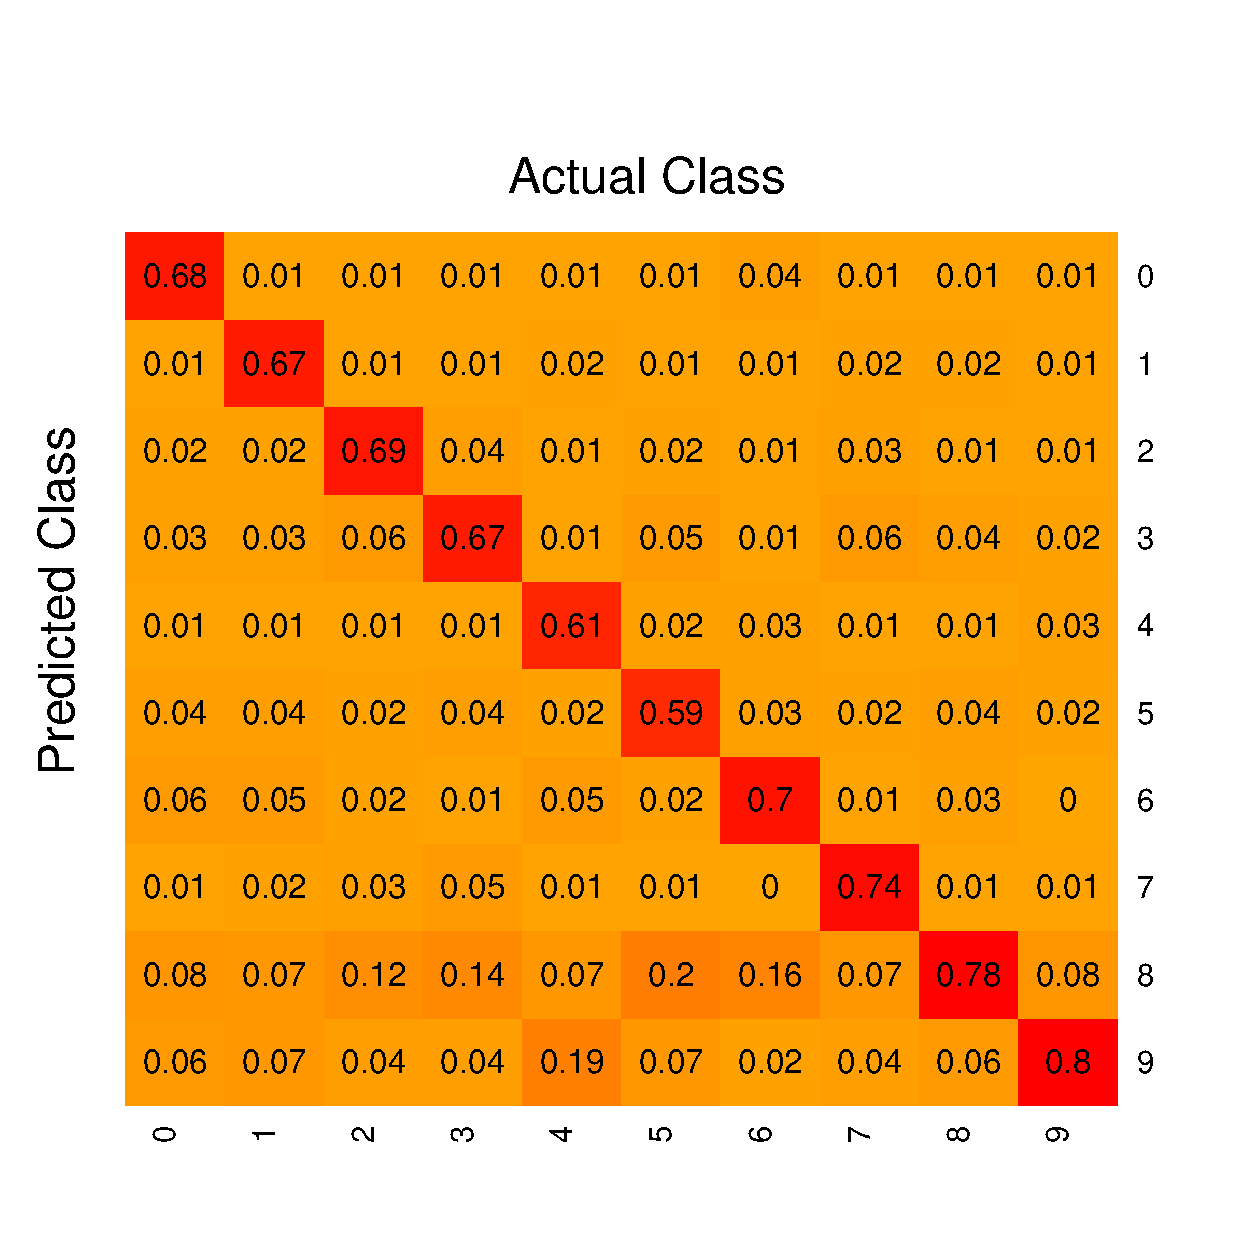
\includegraphics[width=\textwidth]{graphics/tree_confusion_mix}
\caption{Confusion matrix of the prepared data set.}
\label{fig:tree_confus_mixed}
\end{subfigure}
\begin{subfigure}{0.49\textwidth}
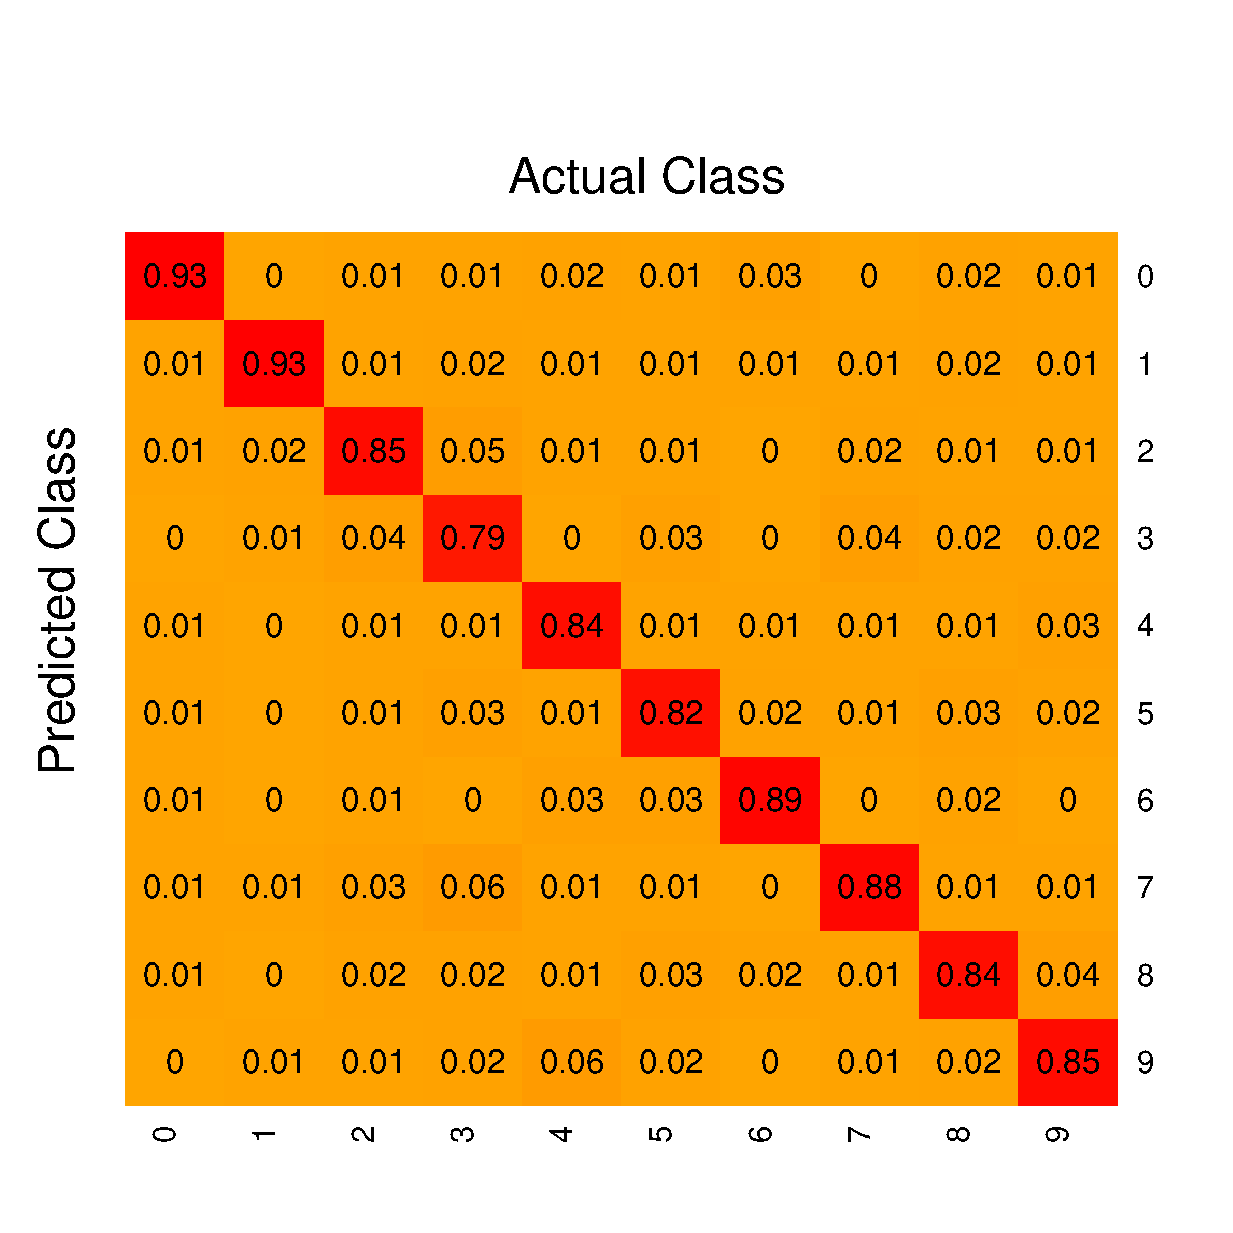
\includegraphics[width=\textwidth]{graphics/tree_confusion_mix2}
\caption{Confusion matrix of the smooth data set.}
\label{fig:tree_confus_mixed_smooth}
\end{subfigure}
\caption{Confusion with all the best parameters for the full dataset on the easy problem.}
\end{figure}

To find the person with the worst handwriting the data set was constructed of all people with one person removed from the training set.
That person was used as test data to see how that person performed.
In figure \ref{fig:tree_performance_all} is the performance shown.
In figure \ref{fig:tree_confus_all} is the average confusion table for all people shown.

\begin{figure}[H]
\centering
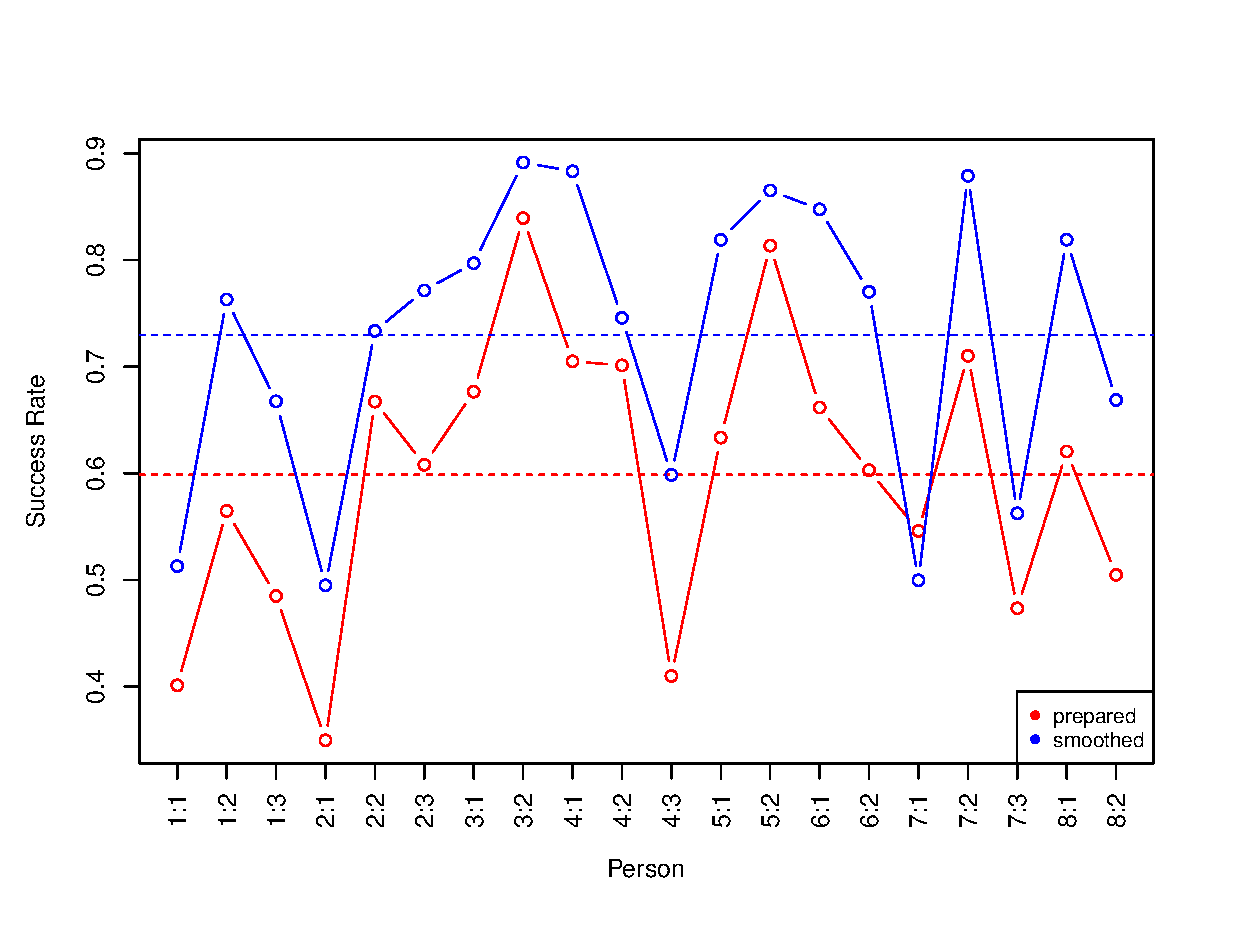
\includegraphics[width=\textwidth]{graphics/tree_performance_all_combined}
% 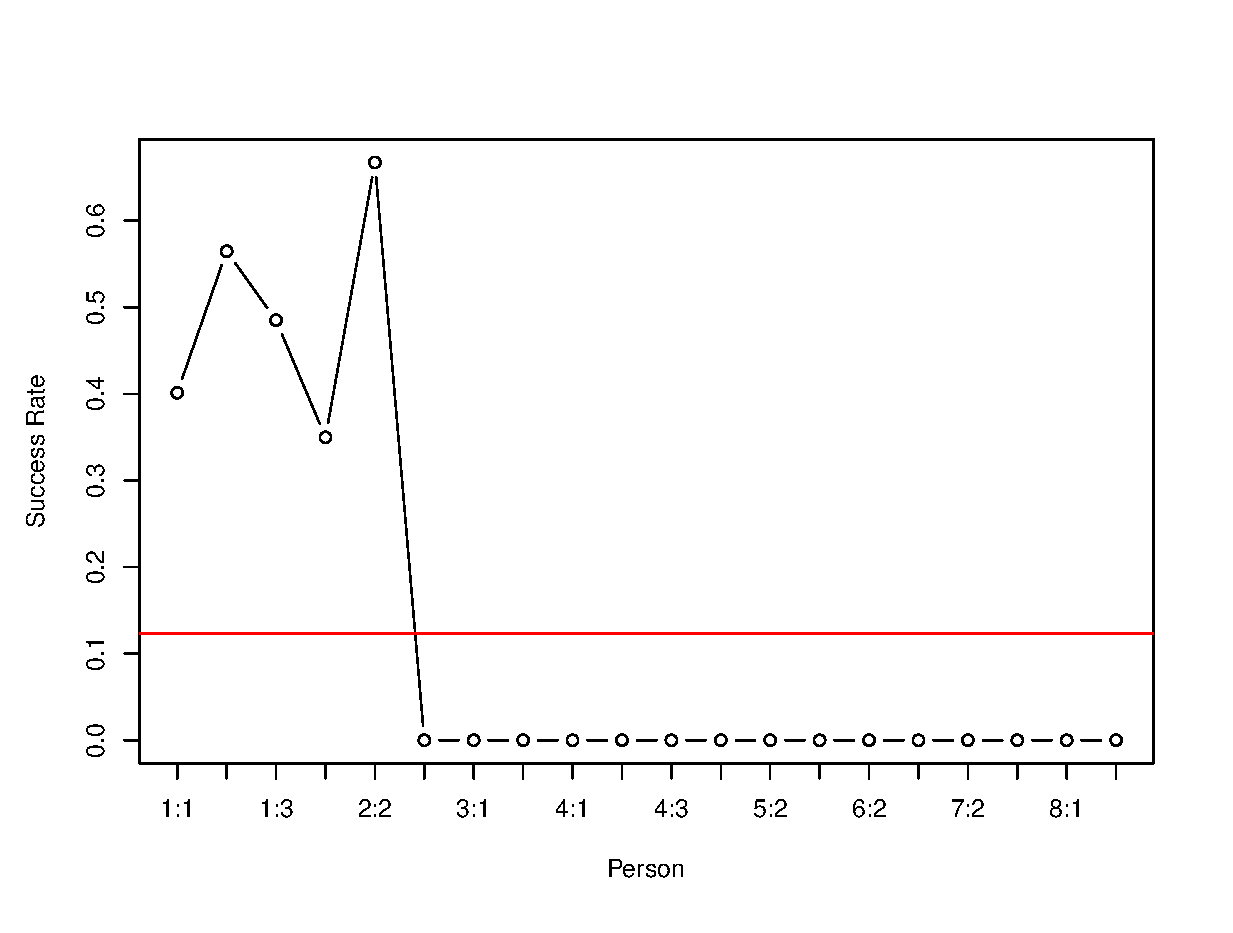
\includegraphics[width=0.47\textwidth]{graphics/tree_performance_all}
% 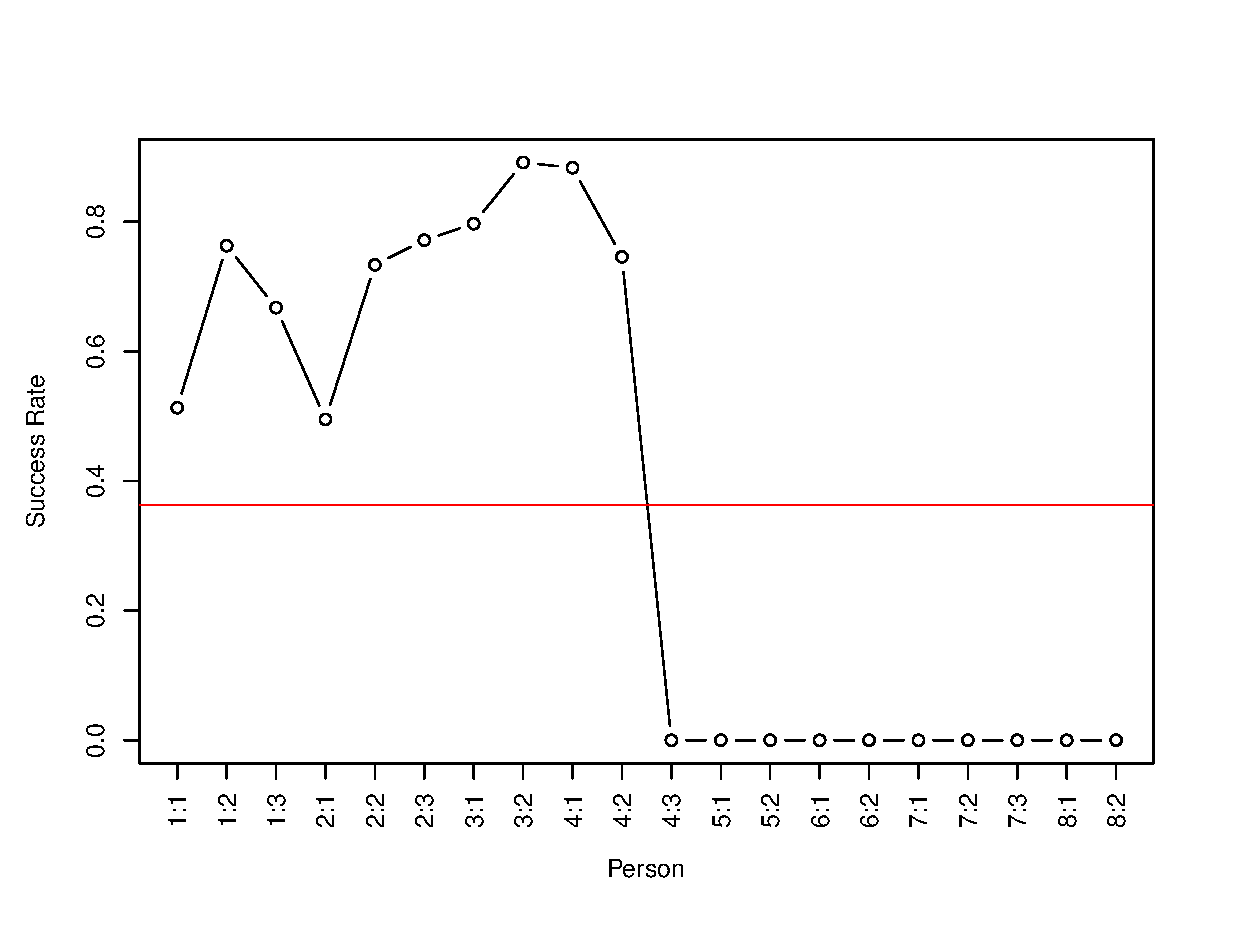
\includegraphics[width=0.47\textwidth]{graphics/tree_performance_all2}
\caption{Confusion with all the best parameters for the full dataset on the hard problem.}
\label{fig:tree_performance_all}
\end{figure}

\begin{figure}[H]
\centering
\begin{subfigure}{0.45\textwidth}
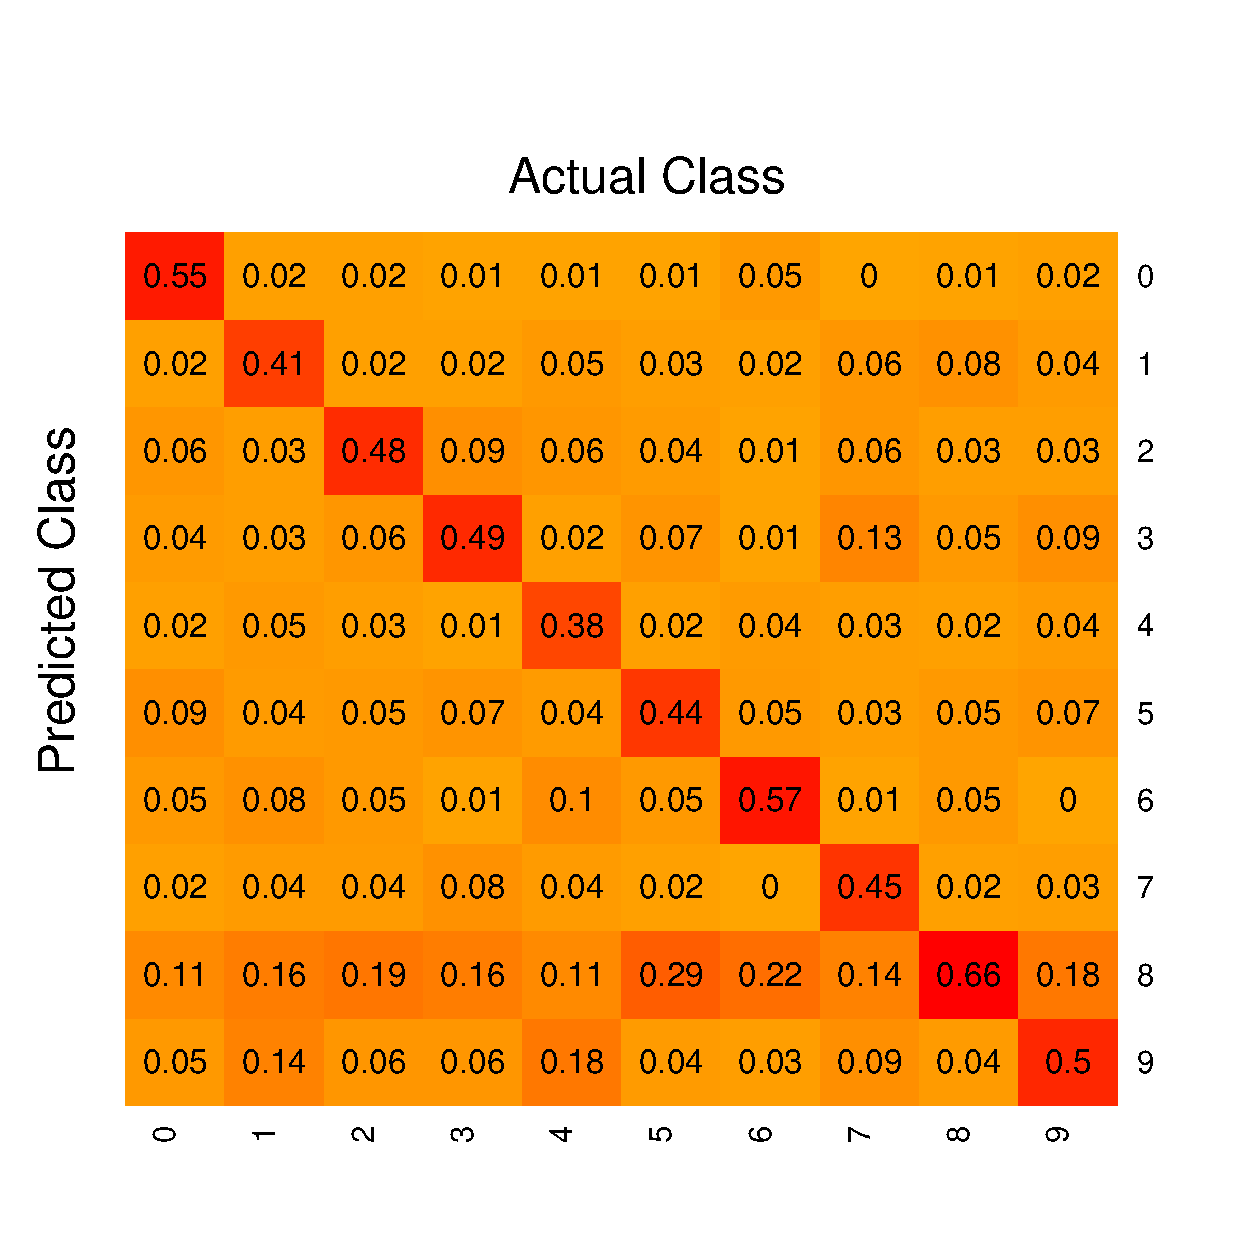
\includegraphics[width=\textwidth]{graphics/tree_confusion_all}
\caption{Prepared data set.}
\end{subfigure}
\begin{subfigure}{0.45\textwidth}
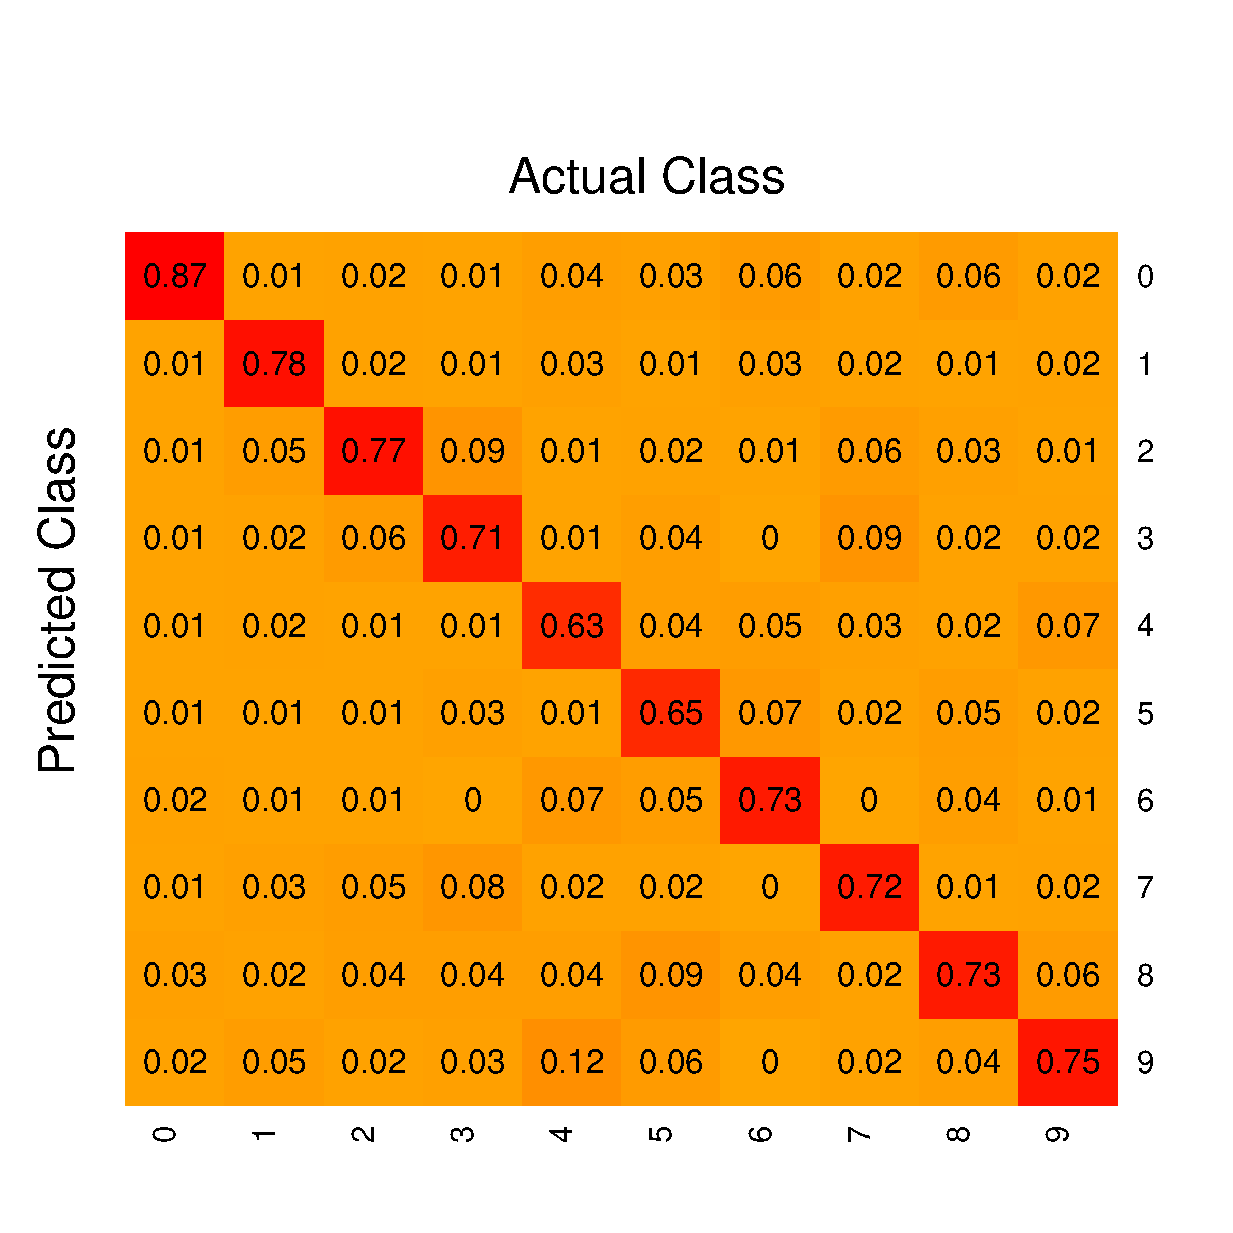
\includegraphics[width=\textwidth]{graphics/tree_confusion_all2}
\caption{Smoothed data set.}
\end{subfigure}
\caption{Confusion matrix for the hard problem}
\label{fig:tree_confus_all}
\end{figure}

To compare the timing performance of the two methods the time it takes to build the two models were measured.
In figure \ref{fig:tree_time_distribution} is the time distribution of both models shown.
As both methods apply a smoothing filter before loading the data this is removed from the time budget as a prepossessing method.
It is seen that the model for the prepared data set is build faster.
Prepossessing is thus a worthwhile optimization when training on a machine with limited resources.
As building a model is only needed once this is seen as less significant than the success rate of the model.
It was measured to take 3056.21 seconds to build the model on the smoothed data set and 2007.00 seconds on the prepared data set.
% 3056.21 s
% 2007.00
% 1942.54 s + 64.46 s

\begin{figure}[H]
\centering
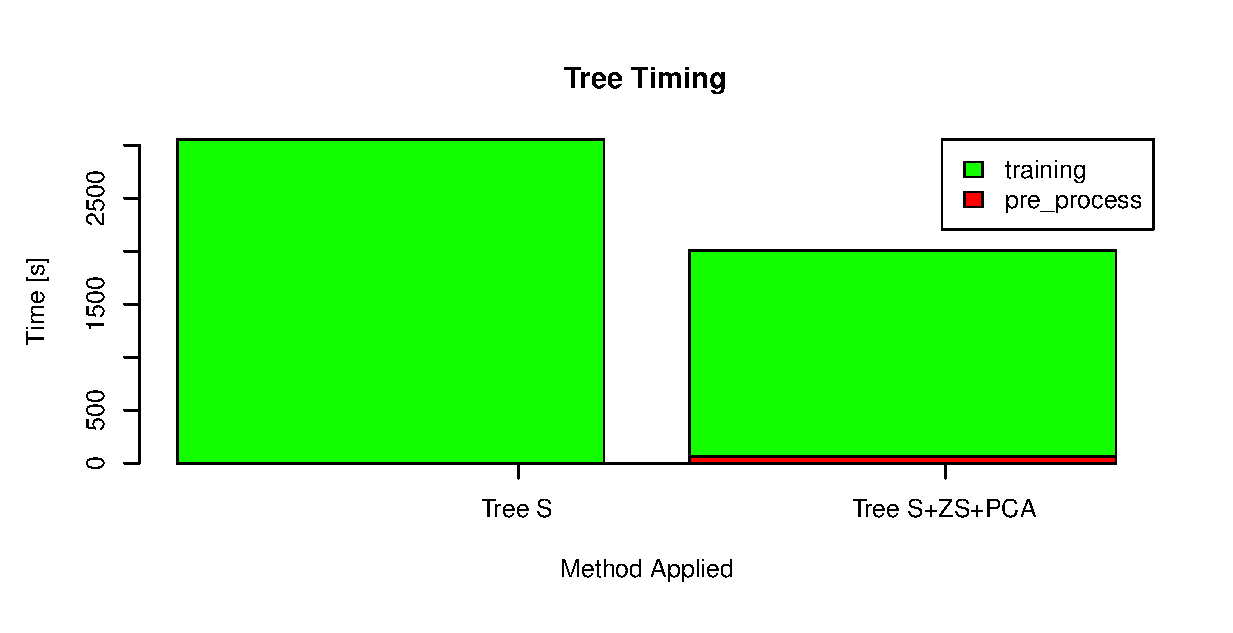
\includegraphics[width=\textwidth]{graphics/algo_compare_timing_tree}
\caption{Time distribution of the prepared data and the smoothed data.}
\label{fig:tree_time_distribution}
\end{figure}